\chapter{Foundations of Multimodal Large Language Models (MLLMs)}


\chapterauthor{Caitlyn}



The purpose of this chapter is to provide an overview of the foundational elements that have led to the development of Multimodal Large Language Models (MLLMs). It covers the evolution of Natural Language Processing (NLP) into Large Language Models (LLMs), explains the unique architecture of MLLMs, discusses the training methodologies and data requirements, and explores the capabilities of MLLMs in cross-modal understanding and visual reasoning.

Multimodal Large Language Models (MLLMs) represent a groundbreaking advancement in the field of artificial intelligence(AI), combining the power of language understanding with visual perception. These sophisticated AI systems are designed to process and comprehend multiple types of data inputs, primarily focusing on text and images, but potentially extending to audio and video as well. To fully grasp the concept of MLLMs, it's essential to break down its components and understand their significance.

At their core, MLLMs are an evolution of Large Language Models (LLMs), which are AI systems trained to understand and generate human language. The term "large" in MLLMs refers to the scale of these models, often containing billions of parameters, which allows them to capture intricate patterns and relationships in data. The "multimodal" aspect is what sets MLLMs apart from traditional LLMs. It indicates the ability to process multiple types of data or "modalities," primarily text and images in the current context.

The significance of MLLMs lies in their ability to bridge the gap between language and vision, much like humans do. When we see a picture, we can easily describe it in words, and conversely, we can visualize a scene based on a textual description. MLLMs aim to replicate this ability, enabling a more comprehensive understanding of given contexts. For instance, when analyzing a news article with accompanying images, an MLLM can provide more accurate insights by considering both the textual content and visual elements.

This enhanced understanding opens up a wide range of applications for MLLMs. They can be used for advanced image captioning, where the model generates detailed descriptions of visual content. Visual question answering is another key application, where MLLMs can respond to queries about specific elements within an image. Some advanced MLLMs are even capable of generating images based on textual descriptions, though this capability is still evolving.

To illustrate the capabilities of MLLMs, let's consider a specific example of visual question answering. Imagine an MLLM is presented with an image of a bustling city street at night, filled with neon signs and people walking. A user might ask, "What time of day is it in this image?" The MLLM, analyzing the visual content, would respond with something like, "It is nighttime in this image. The dark sky and illuminated neon signs indicate that it's evening or night." If asked, "What kind of businesses can you see?" the model might answer, "Based on the neon signs visible in the image, I can see various businesses such as restaurants, bars, and possibly some retail shops. The bright, colorful signs are typical of entertainment districts in cities."

In this example, the MLLM demonstrates several key capabilities. Firstly, it shows an understanding of the visual content of the image, recognizing that it is a night scene in a city. Secondly, it interprets specific elements within the image, such as neon signs, people, and the overall ambiance. Third, it responds to natural language questions about the image content, showcasing its language processing abilities. Finally, it provides detailed, context-aware answers that combine visual understanding with language generation.

The development of MLLMs represents a crucial step towards more human-like AI systems. By processing both text and images, these models can gain a more comprehensive understanding of a given context, much like humans do when interpreting information from multiple sources. This capability enhances human-AI interaction, paving the way for more natural and intuitive exchanges between people and AI systems.

MLLMs possess several key capabilities that set them apart from traditional language models. They can analyze and interpret the content of images, identifying objects, scenes, actions, and emotions described in images. Having a deep understanding of the relationship between textual descriptions and accompanying visuals, they are adept at aligning text and images. Both visual and linguistic information can be comprehended by their visual question-answering abilities. Additionally, MLLMs can generate descriptive captions for images, effectively translating visual information into natural language.

As MLLMs continue to evolve, they promise to revolutionize how we interact with AI systems and how machines understand and interpret the world around us. Their potential applications span various fields, including content creation, education, accessibility, and more. For instance, in education, MLLMs could enhance learning materials by providing detailed explanations of complex diagrams or historical images. In the field of accessibility, they could assist visually impaired individuals by describing the content of images or navigating visual interfaces.

However, it is important to note that the development and application of MLLMs also come with challenges and ethical considerations. These include ensuring the accuracy and fairness of the model's interpretations, addressing potential biases in training data, and considering privacy concerns when processing visual information.

In conclusion, multimodal large language models are a significant step forward in AI technology, bridging the gap between language understanding and visual perception. In the coming years, we can expect to see even more sophisticated applications that utilize MLLMs to enhance our interaction with digital content.

\section{From NLP to LLMs: A Brief Overview}

The history of Multimodal Large Language Models (MLLMs) is deeply rooted in the evolution of Natural Language Processing (NLP). Understanding this progression from traditional NLP methods to modern Large Language Models (LLMs) provides critical insights into how MLLMs were developed and sheds light on their current capabilities and potential future directions.

Early NLP techniques relied heavily on rule-based systems and statistical models. Rule-based systems used handcrafted rules to process and analyze text, which were effective for specific tasks but lacked flexibility and struggled with the complexity of natural language. Statistical models, such as n-grams and Hidden Markov Models (HMMs), introduced probabilistic methods to NLP, allowing for better handling of language variability. However, these models still fell short in capturing deeper linguistic structures.

The integration of machine learning into NLP marked a significant shift, enabling models to learn from data rather than relying solely on predefined rules. Support Vector Machines (SVMs) were used for text classification tasks, leveraging the ability to find optimal decision boundaries in high-dimensional spaces. Naive Bayes, a probabilistic classifier, was popular for tasks like spam detection, utilizing the Bayes theorem to make predictions based on word frequencies.

The rise of deep learning brought transformative changes to NLP, with neural networks enabling more sophisticated language models. Techniques like Word2Vec and GloVe represented words as dense vectors in continuous space, capturing semantic relationships and improving the performance of downstream tasks. Recurrent Neural Networks (RNNs), and their variants like Long Short-Term Memory (LSTM) networks, excelled at processing sequential data, making them suitable for tasks such as language modeling and machine translation. The introduction of attention mechanisms allowed models to focus on relevant parts of the input sequence, enhancing the performance of tasks like translation and summarization.

The development of the Transformer architecture revolutionized NLP, leading to the creation of powerful pre-trained models. The Transformer model, introduced in the paper \cite{vaswani2017attention} utilized self-attention mechanisms to capture dependencies between words, enabling parallel processing and improving scalability. Bidirectional Encoder Representations from Transformers (BERT) leveraged the Transformer architecture to create contextualized word embeddings, achieving state-of-the-art results on various NLP benchmarks. Generative Pre-trained Transformers (GPT) focused on language generation, with models like GPT-3 demonstrating remarkable capabilities in generating coherent and contextually relevant text.

The evolution from LLMs to MLLMs involved integrating visual data with textual data, enabling models to process and understand multiple modalities. Techniques like VisualBERT and VL-BERT extended the BERT architecture to handle both text and images, pre-training on large-scale multimodal datasets to learn joint representations. Cross-modal attention mechanisms allowed models to align and integrate information from different modalities, enhancing their ability to perform tasks like image captioning and visual question answering.

The integration of multimodal data has opened up new possibilities for AI applications. MLLMs can generate detailed descriptions of images, providing valuable assistance in fields like accessibility and content creation. These models can answer questions about images, demonstrating their ability to understand and reason about visual content. MLLMs also enable the creation of rich multimedia content, combining text, images, and audio to produce engaging and informative outputs.

The field of NLP has undergone significant transformations over the past few decades, driven by advancements in computational power, the availability of large-scale datasets, and breakthroughs in machine learning algorithms. This journey can be broadly categorized into several key phases:



\begin{enumerate}
    \item \textbf{Rule-based systems (1950s-1980s):} Early NLP approaches relied heavily on hand-crafted rules and linguistic knowledge bases. While these systems could perform well in narrow domains, they struggled with the complexity and ambiguity of natural language.

    These were handcrafted algorithms that relied on predefined grammatical rules to process text. Though effective in limited contexts, they were inflexible and incapable of handling complex linguistic nuances.

These handcrafted algorithms relied heavily on predefined grammatical rules to process text. Though effective in limited contexts, they were inflexible and incapable of handling complex linguistic nuances. This rigidity hindered their adaptability to diverse scenarios where language context and meaning varied significantly. As a result, these systems struggled with ambiguous or highly contextual inputs, which are common in natural language.

The shortcomings of such rule-based systems, particularly in Natural Language Processing (NLP), highlighted the need for more sophisticated approaches. Rule-based systems were successful in solving specific, well-defined tasks like discourse segmentation or parsing sentences based on syntactic structures, as seen in early attempts like the Linguistic Discourse Model (LDM). These systems used symbolic, syntactic, and semantic rules to process language but required meticulous construction and could only manage relatively straightforward linguistic structures \cite{polanyi2004rule}. Similarly, conventional rule-based expert systems were developed to encode human expertise into conditional rules to address complex decision-making tasks across various domains. These systems were designed with “if-then” logic, enabling machines to simulate human problem-solving \cite{abraham2005rule}.

However, the limitations of these early systems in managing real-world complexity soon became evident. They lacked the flexibility to deal with incomplete or noisy data and were often constrained by the size and scope of their rule base. Despite their limitations, rule-based systems laid the foundation for modern AI, particularly in providing a framework for the development of inference mechanisms like forward and backward chaining. These mechanisms played a crucial role in expert systems, where the aim was to mimic human decision-making processes \cite{abraham2005rule}.

The development of Large Language Models (LLMs) and other machine learning techniques gradually overcame these limitations by using vast amounts of data and statistical methods, allowing for a more nuanced understanding of language and context.

    \item \textbf{Statistical methods (1980s-2000s):} The introduction of statistical techniques, such as Hidden Markov Models and n-gram language models, allowed for more data-driven approaches. These methods could learn patterns from large text corpora, improving performance on tasks like machine translation and speech recognition. This marked a significant departure from rule-based systems, where linguistic expertise and predefined rules dominated.

With statistical models, the focus shifted from handcrafted rules to probabilistic reasoning. For example, HMMs became instrumental in tagging and parsing, where they modeled sequences of observations, such as words or parts of speech, and the probabilities of transitions between states \cite{koehn2009statistical}, \cite{charniak1997statistical}. These models could infer the most likely sequence of syntactic structures or translations based on observed data, making them more adaptable to unseen examples than rule-based systems.

In addition, n-gram models, which represent the probability of a word given its previous words, found success in tasks such as language modeling for speech recognition and machine translation. These models utilized large amounts of data to estimate the likelihood of word sequences, enabling them to predict future words in a sentence with remarkable accuracy \cite{koehn2009statistical}. By calculating probabilities over sequences of tokens, n-gram models helped achieve more fluent and coherent outputs in machine translation \cite{charniak1997statistical}.

Despite their progress, early statistical models had limitations. They were prone to issues like sparse data, where rare word combinations were poorly represented, leading to less accurate predictions. Techniques like smoothing were introduced to mitigate this by assigning small probabilities to unseen word sequences \cite{charniak1997statistical}. Nevertheless, these models laid the groundwork for the more advanced machine learning techniques that would follow, which incorporated deeper linguistic understanding and more sophisticated representations.
    
    \item \textbf{Machine learning era (2000s-2010s):} The rise of machine learning algorithms, particularly supervised learning techniques, improved various NLP tasks significantly. Support Vector Machines (SVM), Decision Trees, and early neural networks became popular for tasks like text classification and named entity recognition. These approaches allowed models to learn from labeled data, where patterns and relationships could be automatically extracted from examples rather than being manually coded as in rule-based systems.

According to \cite{mi2016supervised}, SVMs, for instance, worked by finding hyperplanes that best separated data into different classes, excelling in high-dimensional spaces common in NLP applications. They were especially useful for binary classification tasks, such as determining whether a document belongs to a certain category, like spam detection in emails. Decision Trees, on the other hand, divided data into increasingly smaller subsets based on feature values, creating a tree-like structure that could be easily interpreted and adapted to a variety of tasks.

Early neural networks also began to gain traction during this time, laying the groundwork for the deep learning revolution to follow. These networks were particularly adept at handling complex, nonlinear relationships in data, which was essential for more challenging tasks like machine translation, where simple linear models struggled \cite{conneau2017supervised}. While these early machine learning models marked a significant leap forward compared to rule-based systems, they still faced challenges in generalization and scalability. However, their data-driven nature allowed them to learn from diverse sources and provided a more flexible alternative to the rigid frameworks of earlier approaches.

This transition from manually crafted rules to models capable of learning from data formed the basis for modern NLP approaches, which now rely on even more sophisticated algorithms and architectures, like neural networks with attention mechanisms, to achieve state-of-the-art results\cite{mi2016supervised}, \cite{conneau2017supervised}.
    
    \item \textbf{Deep learning revolution (2010s-present):} The advent of deep learning techniques, especially neural networks with multiple layers, marked a paradigm shift in NLP. This era saw the development of word embeddings, recurrent neural networks (RNNs), and later, transformer-based models, which dramatically improved performance across a wide range of NLP tasks.

    The advent of deep learning techniques, especially neural networks with multiple layers, marked a paradigm shift in NLP. This era saw the development of word embeddings, recurrent neural networks (RNNs), and later, transformer-based models, which dramatically improved performance across a wide range of NLP tasks. Word embeddings, such as Word2Vec and GloVe, allowed models to represent words as dense vectors in continuous space, capturing semantic similarities between words that previous methods like one-hot encoding failed to do \cite{lauriola2022introduction}, \cite{henderson2020unstoppable}. These embeddings enabled models to generalize better and capture context more effectively, leading to significant breakthroughs in tasks like sentiment analysis, machine translation, and text classification.

Recurrent Neural Networks (RNNs), especially their variants like Long Short-Term Memory (LSTM) networks, were introduced to address the challenge of capturing sequential dependencies in language. These models were able to maintain a memory of previous inputs, making them particularly effective for tasks involving temporal or sequential data, such as language modeling, speech recognition, and machine translation \cite{peng2022survey}, \cite{lauriola2022introduction}. However, RNNs faced limitations in handling long-term dependencies due to issues like vanishing gradients.

The limitations of RNNs were later addressed with the development of Transformer-based models, which relied entirely on self-attention mechanisms. The Transformer model, introduced in 2017, revolutionized NLP by allowing for parallelization in training and handling long-range dependencies more effectively than RNNs. This architecture formed the foundation for models like BERT (Bidirectional Encoder Representations from Transformers) and GPT (Generative Pre-trained Transformer), which became the cornerstone of modern NLP applications. These models could be pre-trained on large corpora and fine-tuned for specific tasks, leading to state-of-the-art results in machine translation, question answering, and summarization \cite{lauriola2022introduction}, \cite{henderson2020unstoppable}.
\end{enumerate}

The transition from traditional NLP methods to Large Language Models (LLMs) represents a significant leap in the field's capabilities. LLMs, such as GPT (Generative Pre-trained Transformer) and BERT (Bidirectional Encoder Representations from Transformers), leverage massive amounts of text data and advanced neural network architectures to capture complex linguistic patterns and generate human-like text.

This evolution set the stage for the development of MLLMs, which extend the capabilities of LLMs to handle multiple modalities, particularly integrating vision and language. By understanding the historical context and technological advancements that led to LLMs, we can better appreciate the challenges and opportunities presented by MLLMs in combining textual and visual information processing.

\subsection{Traditional NLP Methods}
Traditional NLP methods focused on rule-based systems and statistical models. These early approaches included:

\textbf{Rule-Based Systems:} These were handcrafted algorithms that relied on predefined grammatical rules to process text. Although effective in limited contexts, they were inflexible and incapable of handling complex linguistic nuances. Despite their limitations, rule-based systems played a crucial role in the evolution of Natural Language Processing and laid the groundwork for more advanced techniques. These systems contributed significantly to our understanding of language structure and the challenges inherent in computational linguistics.

One notable application of rule-based systems was in the development of early machine translation systems. The Georgetown-IBM experiment in 1954, for instance, utilized a rule-based approach to translate Russian sentences into English. While limited in scope, this experiment demonstrated the potential for automated language processing and sparked further research in the field. Rule-based systems also found applications in information extraction tasks. Systems like FASTUS (Finite State Automaton Text Understanding System) employed cascaded finite-state transducers to extract specific information from text. This approach proved effective for well-defined extraction tasks in domains with structured information. Moreover, rule-based systems contributed to the development of formal grammars and parsing techniques. The work on context-free grammars and parsing algorithms, such as the CYK algorithm, provided a foundation for understanding sentence structure and laid the groundwork for more sophisticated natural language understanding systems. The transition from rule-based systems to statistical and machine learning approaches in NLP was gradual. Hybrid systems that combined rules with statistical methods emerged as an intermediate step. These systems attempted to leverage the strengths of both approaches, using rules to capture linguistic knowledge and statistical methods to handle variability and ambiguity in language.

While modern Large Language Models have largely superseded traditional rule-based systems in many NLP tasks, the insights gained from developing and refining rule-based approaches continue to inform current research. The explicit encoding of linguistic knowledge in rules has influenced the design of neural network architectures and the development of linguistically-informed learning objectives in contemporary NLP models.

\textbf{Bag-of-Words and TF-IDF:} These models represented text as a collection of words (bag-of-words), neglecting grammar or word order, but capturing word frequency to identify relevant terms. TF-IDF (Term Frequency-Inverse Document Frequency) improved on this by down-weighting common words and highlighting unique ones. These models, while simplistic in their approach, laid important groundwork for text representation in NLP tasks.

\subsubsection{Bag-of-Words (BoW)}
The Bag-of-Words (BoW) model is a fundamental text representation technique that disregards grammar and word order, instead focusing on the occurrence of words within a document. In this model, each document is represented as a ``bag'' of its words, typically encoded as a vector where each element corresponds to a word in the vocabulary. The value of each element can be binary (indicating presence or absence), the count of occurrences, or some other weighting scheme. Despite its simplicity, BoW has proven effective in various applications, including document classification and information retrieval.

However, the BoW model has limitations. It fails to capture semantic relationships between words and can be biased towards frequently occurring terms that may not be particularly informative. To address these issues, the Term Frequency-Inverse Document Frequency (TF-IDF) model was developed.

\subsubsection{Term Frequency-Inverse Document Frequency (TF-IDF)}
TF-IDF is a statistical measure used to evaluate the importance of a word in a document within a corpus. It comprises two components:

\begin{enumerate}
    \item \textbf{Term Frequency (TF):} This measures how frequently a term appears in a document. It is typically calculated as:
    
    \begin{equation}
        \text{TF}(t,d) = \frac{\text{Number of times term } t \text{ appears in document } d}{\text{Total number of terms in document } d}
    \end{equation}

    \item \textbf{Inverse Document Frequency (IDF):} This measures how important a term is across the entire corpus. It is calculated as:
    
    \begin{equation}
        \text{IDF}(t) = \log\left(\frac{\text{Total number of documents}}{\text{Number of documents containing term } t}\right)
    \end{equation}
\end{enumerate}

The TF-IDF score is then computed by multiplying TF and IDF:

\begin{equation}
    \text{TF-IDF}(t,d) = \text{TF}(t,d) \times \text{IDF}(t)
\end{equation}

This weighting scheme effectively reduces the impact of common words that appear frequently across many documents (like ``the'' or ``and'') while emphasizing words that are more unique to specific documents. As a result, TF-IDF provides a more nuanced representation of document content compared to simple word counts.

Both BoW and TF-IDF models have been widely used in various NLP tasks, including document classification, information retrieval, and as features for more complex machine learning models. While they have largely been superseded by more advanced techniques in many applications, their simplicity and interpretability ensure their continued relevance in certain contexts, particularly in scenarios with limited computational resources or where model explainability is crucial.

\textbf{Early Machine Learning Models:} %The development of machine learning techniques like Naive Bayes, Support Vector Machines (SVMs), and Hidden Markov Models (HMMs) helped NLP models to start generalizing based on statistical relationships, though they were still limited in their ability to capture deeper linguistic context.

Early machine learning models revolutionized Natural Language Processing (NLP), introducing statistical approaches that could learn patterns from data. These models, while still limited in their ability to capture deep linguistic context, represented a crucial step forward in the evolution of NLP techniques. Notable among these early models were Naive Bayes classifiers, which applied probabilistic methods to text classification; Support Vector Machines (SVMs), which excelled in high-dimensional spaces typical of text data; and Hidden Markov Models (HMMs), which proved particularly effective for sequential data processing in tasks such as part-of-speech tagging. These approaches laid the groundwork for more advanced techniques, demonstrating the potential of statistical methods in language processing and paving the way for the deep learning revolution in NLP.

\subsection{Rise of Large Language Models (LLMs)}
To overcome the limitations of traditional methods, Large Language Models (LLMs) were developed, which leveraged deep learning architectures such as neural networks. In NLP, LLMs represent a paradigm shift from traditional rule-based and statistical approaches to more sophisticated, data-driven approaches. This evolution was catalyzed by advancements in deep learning architectures, increased computational capabilities, and the availability of vast amounts of textual data.

\subsubsection{Neural Network Foundations}
The foundation for LLMs was laid with the advent of neural network-based models in NLP. These models, particularly those utilizing deep learning techniques, demonstrated an unprecedented ability to capture complex linguistic patterns and relationships. Unlike their predecessors, neural models could automatically learn hierarchical representations of language, reducing the need for manual feature engineering.

\subsubsection{Emergence of Transformer Architecture}
A pivotal moment in the development of LLMs was the introduction of the Transformer architecture by Vaswani et al. (2017) in their seminal paper "Attention is All You Need". The Transformer's self-attention mechanism allowed models to process input sequences in parallel, capturing long-range dependencies more effectively than previous sequential models like Recurrent Neural Networks (RNNs) and Long Short-Term Memory (LSTM) networks.

\subsubsection{Pre-training and Transfer Learning}
The concept of pre-training on large corpora of unlabeled text data, followed by fine-tuning on specific tasks, became a cornerstone in the development of LLMs. This approach, exemplified by models like BERT (Bidirectional Encoder Representations from Transformers) by Devlin et al. (2018), allowed models to acquire general language understanding that could be transferred to a wide range of NLP tasks with minimal task-specific training.

\subsubsection{Scaling Up: From BERT to GPT}
The progression from BERT to models like GPT (Generative Pre-trained Transformer) by OpenAI marked a significant increase in model size and capability. GPT-3, introduced by Brown et al. (2020), with its 175 billion parameters, demonstrated remarkable few-shot learning abilities across various language tasks, approaching human-level performance in some cases.

\subsubsection{Multimodal Extensions}
As LLMs continued to evolve, researchers began exploring ways to extend their capabilities beyond text, leading to the development of multimodal models. These models, capable of processing both textual and visual information, represent the next frontier in AI, bridging the gap between language understanding and visual perception.

\subsubsection{Ethical and Computational Considerations}
The rise of LLMs has also brought forth important discussions regarding the ethical implications of these powerful models, including issues of bias, privacy, and the environmental impact of training such large-scale systems. Additionally, the computational resources required for training and deploying LLMs have spurred research into more efficient architectures and training methodologies.

%In conclusion, the rise of Large Language Models has fundamentally transformed the landscape of NLP, enabling unprecedented advances in language understanding and generation. 
%As these models continue to evolve, they promise to push the boundaries of artificial intelligence, opening new avenues for research and applications in human-computer interaction.

\textbf{Word Embeddings:} Techniques such as Word2Vec and GloVe introduced the idea of embedding words in a continuous vector space, where the distance between words reflects their semantic relationships. This allowed for a more nuanced understanding of language. Word embeddings represent a significant advancement in the field of NLP, offering a sophisticated method for representing words as dense vectors in a continuous vector space. This approach, pioneered by techniques such as Word2Vec (\cite{mikolov2013efficient}) and GloVe (\cite{pennington2014glove}), revolutionized the way machines process and understand language by capturing semantic relationships between words in a numerical format.

The fundamental principle behind word embeddings is the distributional hypothesis, which posits that words appearing in similar contexts tend to have similar meanings. By leveraging this hypothesis, word embedding models analyze large corpora of text to learn vector representations of words. These vectors typically have dimensions ranging from 50 to 300, allowing for a rich representation of semantic and syntactic properties.

One of the most notable characteristics of word embeddings is their ability to capture semantic relationships in vector space. For instance, in a well-trained embedding space, the vector operation "king" - "man" + "woman" would result in a vector close to "queen". This property enables machines to perform analogical reasoning and understand complex linguistic relationships.

Word embeddings have several advantages over traditional one-hot encoding methods:
\begin{enumerate}
    \item \textbf{Dimensionality Reduction:} They provide a dense representation of words, significantly reducing the dimensionality compared to sparse representations like one-hot encoding.
    \item \textbf{Semantic Similarity:} The cosine similarity between word vectors correlates with semantic similarity, allowing for meaningful comparisons between words.
    \item \textbf{Generalization:} Word embeddings enable models to generalize better to unseen words by leveraging the semantic relationships learned during training.
    \item \textbf{Transfer Learning:} Pre-trained word embeddings can be used as input features for various NLP tasks, facilitating transfer learning and improving performance on downstream tasks.
\end{enumerate}

Despite their advantages, word embeddings also have limitations. They struggle with polysemy (words with multiple meanings) and require large amounts of training data to learn accurate representations. Additionally, they are static, meaning the same word always has the same embedding regardless of context.

Subsequent developments, such as contextual embeddings (e.g., ELMo, BERT), have addressed some of these limitations by generating dynamic word representations based on the surrounding context. Nevertheless, the introduction of word embeddings marked a pivotal moment in NLP, laying the groundwork for many of the advanced language models we see today.

\textbf{Recurrent Neural Networks (RNNs) and Long Short-Term Memory (LSTM):} These models improved sequential data processing by retaining information over longer time steps, making them useful for tasks like language translation and text generation.

Recurrent Neural Networks (RNNs) and Long Short-Term Memory (LSTM) networks represent significant advancements in sequential data processing, particularly in the domain of Natural Language Processing (NLP). These architectures addressed the limitations of traditional feedforward neural networks by introducing mechanisms to retain information over extended sequences, making them particularly well-suited for tasks such as language translation, text generation, and sentiment analysis.

\textbf{Recurrent Neural Networks (RNNs):}
RNNs introduced a novel approach to processing sequential data by incorporating feedback connections, allowing information to persist through time steps. This recurrent structure enables the network to maintain a form of 'memory' about previous inputs, which is crucial for understanding context in language processing tasks. The basic RNN architecture consists of a hidden state that is updated at each time step, taking into account both the current input and the previous hidden state.

Mathematically, the hidden state $h_t$ at time $t$ is computed as:
\begin{equation}
    h_t = f(W_{hh}h_{t-1} + W_{xh}x_t + b_h)
\end{equation}

Where $W_{hh}$ and $W_{xh}$ are weight matrices, $x_t$ is the input at time $t$, $b_h$ is a bias term, and $f$ is typically a non-linear activation function such as tanh or ReLU.

Despite their ability to capture temporal dependencies, traditional RNNs suffer from the vanishing gradient problem, which limits their effectiveness in learning long-range dependencies. This limitation led to the development of more sophisticated architectures, notably the Long Short-Term Memory networks.

\textbf{Long Short-Term Memory (LSTM):}
LSTM networks, introduced by \cite{hochreiter1997long}, were designed to mitigate the vanishing gradient problem inherent in standard RNNs. LSTMs incorporate a more complex internal structure, featuring a memory cell and three gating mechanisms: input gate, forget gate, and output gate. These gates regulate the flow of information into, out of, and within the memory cell, allowing the network to selectively remember or forget information over long sequences.

The LSTM update equations are as follows:

\begin{align}
f_t &= \sigma(W_f \cdot [h_{t-1}, x_t] + b_f) \\
i_t &= \sigma(W_i \cdot [h_{t-1}, x_t] + b_i) \\
\tilde{C}_t &= \tanh(W_C \cdot [h_{t-1}, x_t] + b_C) \\
C_t &= f_t * C_{t-1} + i_t * \tilde{C}_t \\
o_t &= \sigma(W_o \cdot [h_{t-1}, x_t] + b_o) \\
h_t &= o_t * \tanh(C_t)
\end{align}

Where $\sigma$ denotes the sigmoid function, $*$ represents element-wise multiplication, $[h_{t-1}, x_t]$ is the concatenation of the previous hidden state and current input, and $W_f$, $W_i$, $W_C$, $W_o$ are weight matrices for the forget gate, input gate, cell state, and output gate, respectively.

The sophisticated gating mechanism of LSTMs allows them to capture long-term dependencies more effectively than standard RNNs. This capability has made LSTMs particularly successful in various NLP tasks, including machine translation, speech recognition, and text summarization.

Both RNNs and LSTMs have played pivotal roles in advancing the field of NLP, serving as foundational architectures for many state-of-the-art models. Their ability to process sequential data and capture temporal dependencies has been instrumental in improving performance on a wide range of language-related tasks. While more recent architectures like Transformers have surpassed RNNs and LSTMs in many applications, the principles underlying these recurrent models continue to influence the design of modern NLP systems.

\textbf{Transformers and BERT:} The introduction of the Transformer architecture in the paper Attention is All You Need revolutionized NLP. Transformers enabled models like BERT (Bidirectional Encoder Representations from Transformers) to perform well across various NLP tasks by utilizing self-attention mechanisms to capture contextual relationships between words.

The Transformer architecture, introduced by Vaswani et al. (2017) in their seminal paper "Attention is All You Need," marked a paradigm shift in natural language processing. This model eschews recurrence and convolutions entirely in favor of self-attention mechanisms, allowing for more efficient parallel processing and improved modeling of long-range dependencies in sequential data.

At the core of the Transformer architecture is the multi-head attention mechanism. This mechanism allows the model to jointly attend to information from different representation subspaces at different positions. Mathematically, for a given query Q, key K, and value V, the attention function is computed as:
\begin{equation}
    Attention(Q, K, V) = softmax(\frac{QK^T}{\sqrt{d_k}})V
\end{equation}


Where $d_k$ is the dimension of the key vectors. The multi-head attention extends this by linearly projecting the queries, keys, and values h times with different learned projections, applying attention to each projection in parallel, and concatenating the results.

The Transformer architecture consists of an encoder and a decoder, each composed of a stack of identical layers. Each layer in the encoder contains two sub-layers: a multi-head self-attention mechanism and a position-wise fully connected feed-forward network. The decoder is similar but includes an additional sub-layer that performs multi-head attention over the output of the encoder stack. Residual connections and layer normalization are employed around each sub-layer to facilitate training of deep models.

Building upon the Transformer architecture, Bidirectional Encoder Representations from Transformers (BERT), introduced by Devlin et al. (2018), further revolutionized NLP by introducing a powerful pre-training approach. BERT is designed to pre-train deep bidirectional representations from unlabeled text by jointly conditioning on both left and right context in all layers.

BERT's pre-training involves two unsupervised tasks:

1. Masked Language Model (MLM): A certain percentage of input tokens are masked, and the model is trained to predict these masked tokens based on the context provided by the non-masked tokens.

2. Next Sentence Prediction (NSP): The model is trained to predict whether a given sentence follows another in the original text, helping it understand the relationship between sentences.

The pre-trained BERT model can then be fine-tuned with just one additional output layer to create state-of-the-art models for a wide range of NLP tasks, such as question answering, sentiment analysis, and named entity recognition, without substantial task-specific architecture modifications.

BERT's bidirectional nature, enabled by the Transformer's self-attention mechanism, allows it to capture context from both directions, leading to a more nuanced understanding of language compared to previous unidirectional models. This bidirectional context is particularly crucial for tasks that require a deep understanding of language semantics and context.

The success of BERT has spawned numerous variants and improvements, such as RoBERTa, ALBERT, and T5, each pushing the boundaries of what's possible in NLP. These models have not only advanced the state-of-the-art in various NLP benchmarks but have also paved the way for more efficient and effective transfer learning in language understanding tasks.


\textbf{GPT and the Rise of Generative Models:} Generative Pre-trained Transformers (GPT) introduced a new paradigm for language generation, where pre-trained models could be fine-tuned on specific tasks. This paved the way for GPT-3 and similar models, which exhibited unprecedented language generation capabilities. LLMs like these are foundational to MLLMs, which extend similar architectures to multimodal tasks. The Generative Pre-trained Transformer (GPT) series, introduced by OpenAI, represents a significant milestone in the evolution of language models and generative AI. These models, built upon the Transformer architecture, have progressively pushed the boundaries of natural language processing and generation capabilities.

In 2018, GPT demonstrated the effectiveness of unsupervised pre-training on large corpora of text, followed by fine-tuning. With this approach, the model acquired a broad understanding of language structure and content, allowing it to be adapted to various downstream tasks with minimal task-specific training. The subsequent iterations, GPT-2 and GPT-3, marked substantial advancements in scale and capability. GPT-3, in particular, with its 175 billion parameters, exhibited remarkable few-shot and zero-shot learning abilities across a wide range of language tasks. This model demonstrated an unprecedented capacity for task generalization, often performing competitively with fine-tuned models without any task-specific training.

Several years after the success of the GPT series, NLP applications and research have witnessed a paradigm shift. Key aspects of this shift include:
\\
1. Scale as a Driver of Capability: The GPT models demonstrated that increasing model size and training data volume could lead to qualitative improvements in language understanding and generation.
\\
2. Emergence of In-context Learning: Large language models like GPT-3 exhibited the ability to perform tasks based solely on instructions or examples provided in the input prompt, without fine-tuning.
\\
3. Versatility and Adaptability: These models showed proficiency in a diverse array of tasks, from translation and summarization to code generation and creative writing.
\\
4. Ethical and Societal Implications: The powerful capabilities of these models raised important questions about their potential impact on society, including concerns about misinformation, bias, and the future of human-AI interaction.
\\
With the advent of GPT and similar models, multimodal systems and language models have become even more advanced. The line between different types of AI systems has further blurred with subsequent developments like GPT-4, which incorporates multimodal capabilities.

These advancements in generative models have profound implications for MLLMs. The principles of large-scale pre-training, the ability to understand and generate human-like text, and the capacity for few-shot learning are all crucial elements that MLLMs build upon. By extending these capabilities to include visual inputs, MLLMs represent the next frontier in AI's ability to understand and interact with the world in a more human-like manner.

\section{Architecture of MLLMs}

%MLLMs build on the foundational architecture of LLMs by incorporating additional components for handling multimodal data. In this section, we explore the core architectural components that enable MLLMs to process both text and visual data.

The architecture of Multimodal Large Language Models (MLLMs) represents a significant advancement in artificial intelligence, combining the strengths of language models with the ability to process and understand visual information. This integration allows MLLMs to perform complex tasks that require reasoning across both textual and visual domains.

At its core, the architecture of MLLMs is designed to bridge the gap between language understanding and visual perception. This is achieved through a carefully crafted combination of neural network components, each specialized for different aspects of multimodal processing. The key components of MLLM architecture typically include several interconnected elements working in harmony.

A crucial part of the MLLM architecture is the visual encoder, responsible for processing and encoding visual inputs. This component often utilizes convolutional neural networks (CNNs) or more advanced architectures like Vision Transformers (ViT) to extract meaningful features from images or video frames. Working alongside the visual encoder is the language encoder, similar to traditional language models. This component processes textual inputs and is typically based on the Transformer architecture, allowing for contextual understanding of text.

Central to the MLLM's ability to handle multimodal data is the multimodal fusion module. This critical component integrates the information from both visual and textual modalities, creating a unified representation that captures the relationships between visual and linguistic features. Complementing the fusion module are cross-modal attention mechanisms, which enable the model to attend to relevant parts of one modality while processing the other. For instance, when answering a question about an image, the model can focus on specific image regions that are most relevant to the question.

Finally, the decoder generates outputs based on the fused multimodal representations. Depending on the task, this could involve generating text, classifying images, or producing other forms of multimodal output. The seamless integration of these components allows MLLMs to perform a wide range of tasks that require joint understanding of visual and textual information. This architectural design enables MLLMs to not only process each modality independently but also to reason about the relationships between them, leading to more sophisticated and human-like understanding of multimodal inputs.
\\
\textbf{Transformer Backbone:} 
\begin{figure}
    \centering
    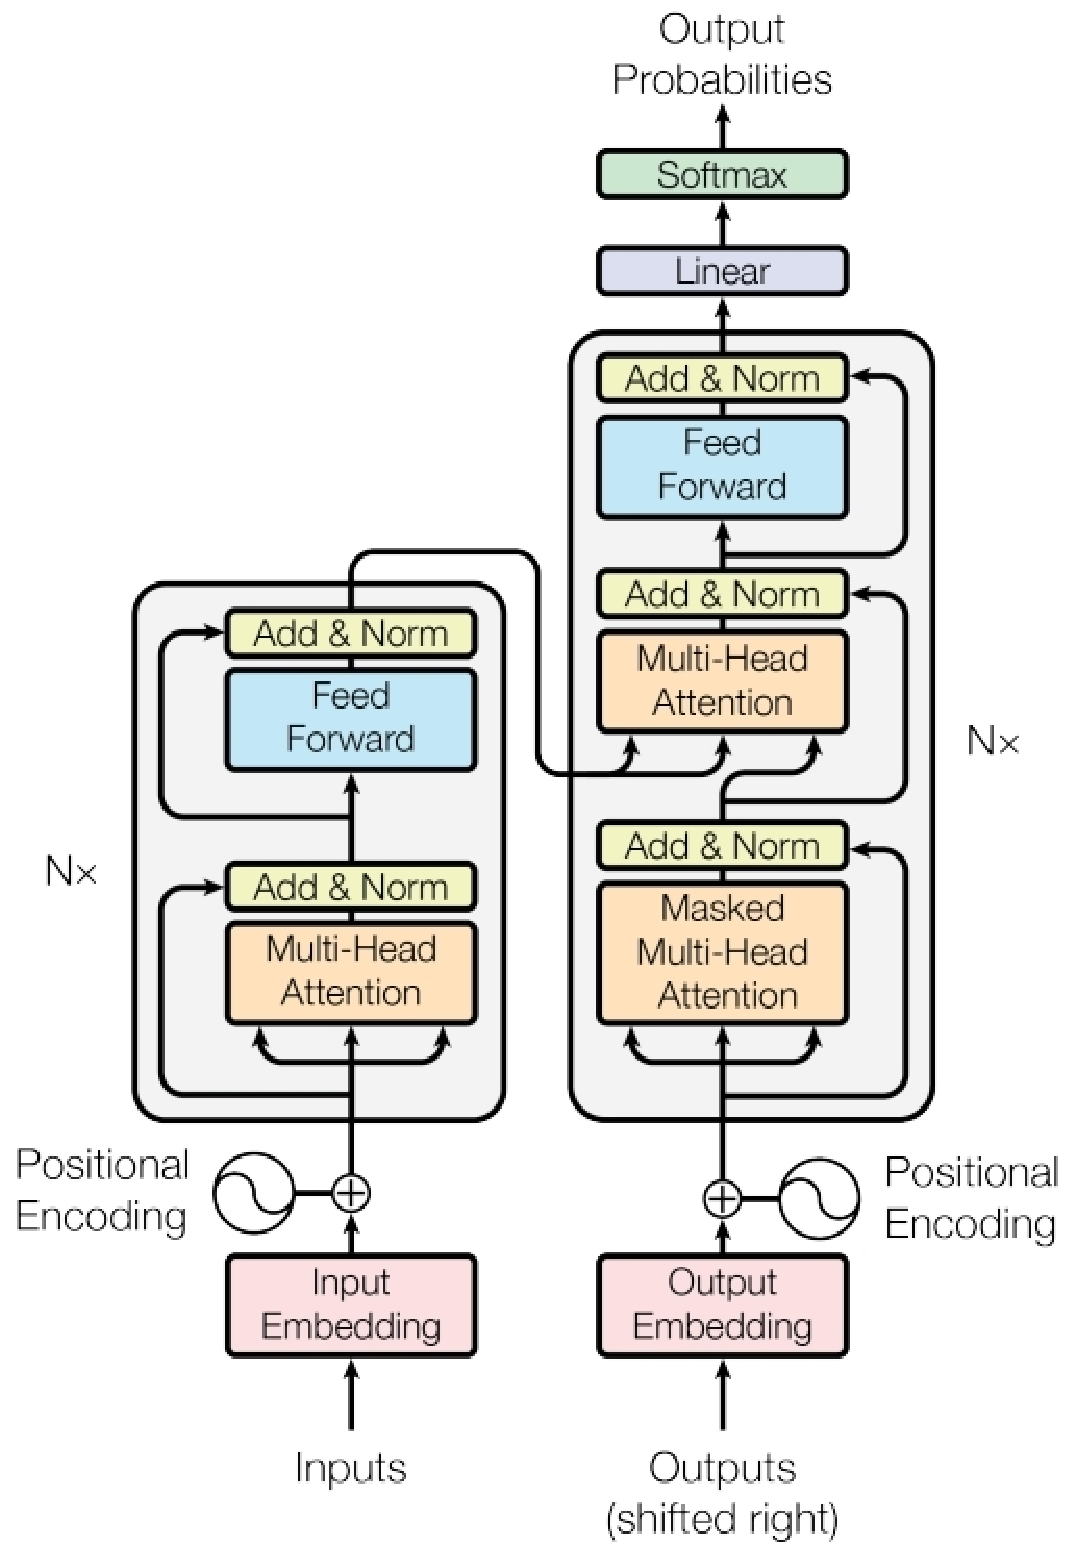
\includegraphics[width=0.4\linewidth]{chapter2/transformer.pdf}
    \caption{Transformer Backbone}
    \label{fig:transformer}
\end{figure}
\\
MLLMs typically rely on the Transformer architecture, which uses self-attention to understand the relationships between data elements, whether they are words or image patches. The Transformer model’s ability to handle sequential and parallel information makes it ideal for multimodal tasks.

The Transformer architecture, introduced by Vaswani et al. (2017), serves as the fundamental backbone for MLLMs, providing a powerful mechanism for processing both textual and visual information. This architecture's core strength lies in its self-attention mechanism, which allows the model to dynamically focus on relevant parts of the input, regardless of their position in the sequence.

MLLMs benefit greatly from the Transformer's versatility. Multimodal tasks benefit from its ability to handle both sequential and parallel data (like text). In order to understand the nuanced relationships between visual and textual elements, the self-attention mechanism allows the model to capture long-range dependencies and complex relationships.

The Transformer's architecture typically consists of multiple layers of self-attention and feed-forward neural networks. In MLLMs, this structure is often adapted to include:
\\
1. Encoder layers: These process the input data, whether it's text tokens or visual features, and create contextualized representations.
\\
2. Decoder layers: These generate output based on the encoded representations, often incorporating cross-attention mechanisms to attend to relevant parts of the input.
\\
3. Multi-head attention: This allows the model to attend to different aspects of the input simultaneously, enhancing its ability to capture diverse relationships in multimodal data.
\\
4. Position encodings: These are crucial for maintaining spatial or sequential information, especially important when dealing with image patches or text sequences.
\\
Scalability is another factor that contributes to the Transformer's popularity among MLLMs. As demonstrated by models like GPT-3 and CLIP, increasing the size of Transformer-based models often leads to improved performance and generalization capabilities. This scalability allows MLLMs to leverage vast amounts of multimodal data effectively, leading to more robust and versatile models.

Furthermore, the Transformer's architecture facilitates efficient parallel processing, making it well-suited for handling the computational demands of large-scale multimodal tasks. This efficiency is crucial when processing high-dimensional inputs like images alongside text.


\textbf{Multimodal Embedding:} 
\begin{figure}
    \centering
    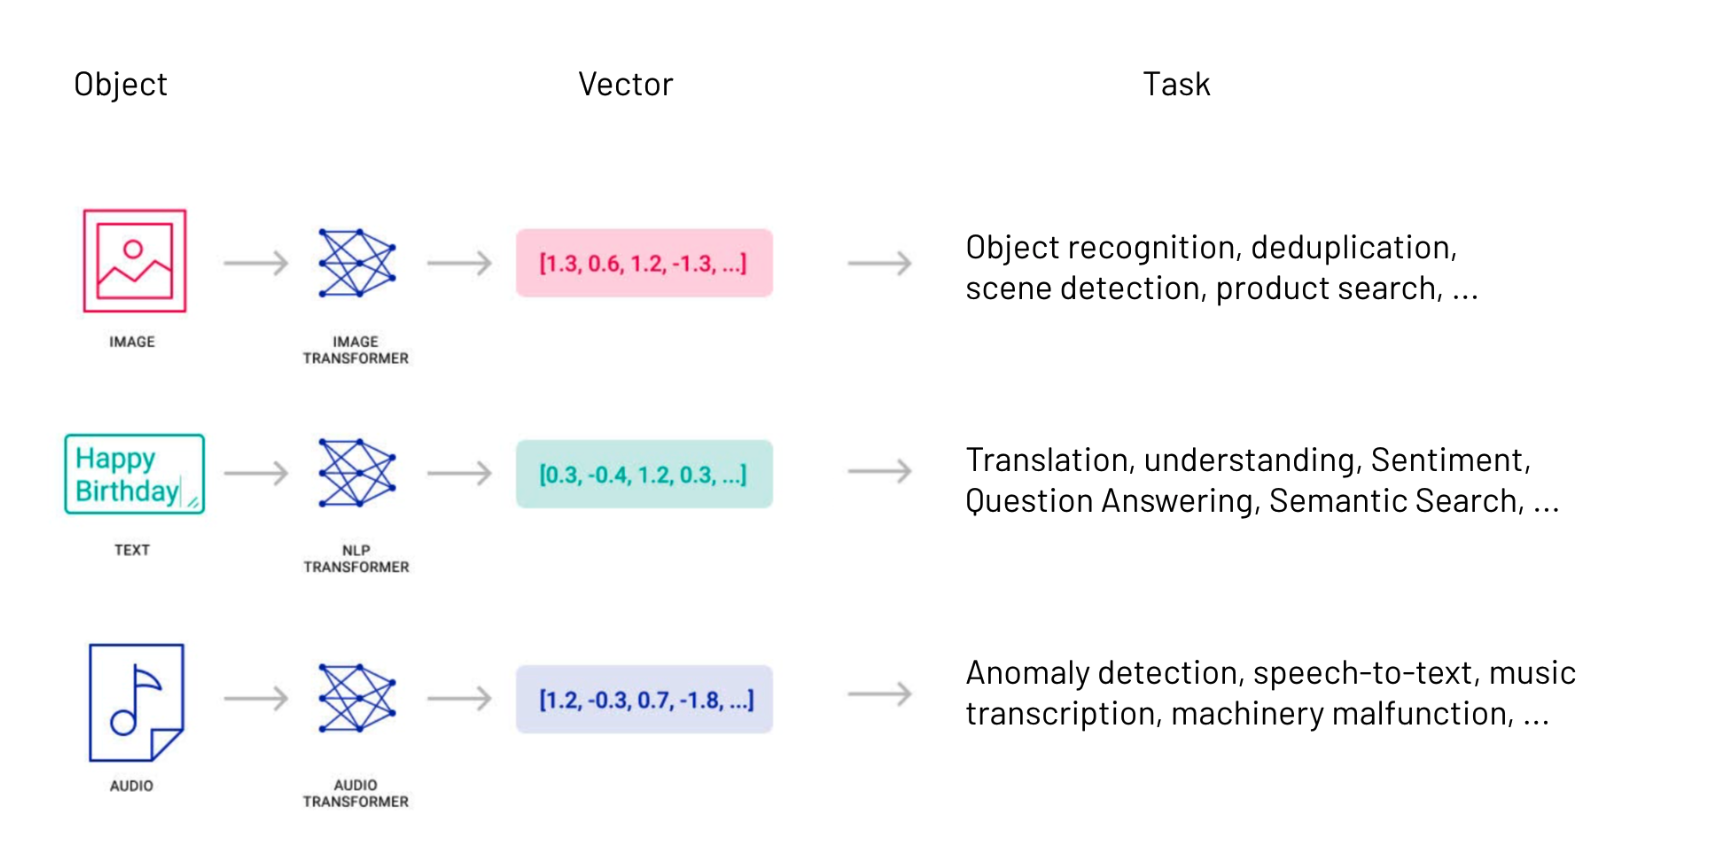
\includegraphics[width=1.0\linewidth]{chapter2/multimodal_embeddings.png}
    \caption{Multimodal Embeddings}
    Source: \url{https://www.twelvelabs.io/blog/multimodal-embeddings}
    \label{fig:multimodal_embeddings}
\end{figure}
One of the key features of MLLMs is their ability to embed both text and visual information into a unified space. This allows the model to reason about both modalities in a consistent manner, ensuring that relationships between visual and textual data can be leveraged effectively.

Multimodal embedding is a crucial component in the architecture of MLLMs, enabling these models to represent and reason about diverse types of information within a unified computational framework. This technique involves projecting data from different modalities—primarily text and images in the context of MLLMs—into a shared, high-dimensional vector space. The resulting embeddings capture semantic relationships not only within each modality but also across modalities, facilitating more sophisticated cross-modal reasoning and analysis.

The process of creating multimodal embeddings typically involves several key steps:
\\
1. Modality-Specific Encoding: Initially, each input modality is processed through specialized encoders. For textual data, this often involves tokenization followed by embedding through techniques like word2vec or more advanced contextual embedding methods. Visual data is typically encoded using convolutional neural networks (CNNs) or Vision Transformers (ViT) to extract salient features.
\\
2. Dimensionality Alignment: The embeddings from different modalities are often of different dimensionalities. A crucial step is to project these embeddings into a common dimensional space, usually through learnable linear transformations or more complex neural network layers.
\\
3. Joint Representation Learning: The aligned embeddings are then further processed to create a truly joint representation. This often involves attention mechanisms or fusion layers that allow the model to learn complex interactions between the modalities.
\\
4. Contrastive Learning: Many state-of-the-art MLLMs employ contrastive learning techniques during training. This approach encourages the model to produce similar embeddings for semantically related text-image pairs while pushing apart unrelated pairs in the embedding space.
\\
5. Fine-tuning for Downstream Tasks: The joint embeddings are then fine-tuned on specific downstream tasks, allowing the model to adapt its representations for particular applications while retaining the general cross-modal understanding gained during pretraining.
\\
The effectiveness of multimodal embeddings in MLLMs is evidenced by their performance on various tasks requiring cross-modal understanding. For instance, in image-text retrieval tasks, these embeddings enable the model to find semantically relevant images given a textual query, and vice versa. In visual question answering, the joint embedding space allows the model to reason about textual questions in the context of visual information.

Moreover, recent research has shown that multimodal embeddings can capture nuanced relationships between concepts across modalities. For example, they can represent abstract concepts that are difficult to visualize directly but are often associated with certain visual patterns or contexts. This capability enables MLLMs to perform more human-like reasoning tasks, such as visual commonsense inference or generating creative descriptions of images.

However, creating effective multimodal embeddings also presents several challenges. These include dealing with the semantic gap between modalities, handling the different statistical properties of visual and textual data, and ensuring that the embeddings generalize well across diverse tasks and domains. Ongoing research in this area focuses on developing more sophisticated embedding techniques, exploring ways to incorporate additional modalities, and improving the interpretability of these high-dimensional representations.


\textbf{Cross-Attention Layers:} To enable interaction between text and images, MLLMs often employ cross-attention mechanisms. These layers allow the model to focus on relevant parts of an image when processing a piece of text (or vice versa), enhancing the ability to understand the relationships between the two.

Cross-attention layers are a fundamental component of MLLMs, facilitating the intricate interplay between textual and visual modalities. These layers enable the model to dynamically focus on relevant aspects of one modality while processing information from the other, thereby enhancing the model's capacity to understand and reason about multimodal inputs.

The mechanism of cross-attention is derived from the self-attention concept introduced in the Transformer architecture. However, unlike self-attention, which operates within a single modality, cross-attention allows the model to attend to information across different modalities. In the context of MLLMs, this typically involves attention between textual and visual representations.

The cross-attention process can be formalized as follows:

Let Q represent the query vectors from one modality (e.g., text), and K and V represent the key and value vectors from another modality (e.g., image). The cross-attention operation can be expressed as:
\begin{equation}
    Attention(Q, K, V) = softmax(Q{K^T} / \sqrt{d_k})V.
\end{equation}
Where $d_k$ is the dimensionality of the key vectors, and the softmax operation is applied row-wise.

This formulation allows the model to compute attention weights that determine the relevance of each element in one modality to each element in the other modality. For instance, when processing a textual query about an image, the cross-attention layer enables the model to focus on specific regions of the image that are most pertinent to the query.

The benefits of cross-attention layers in MLLMs are multifold:
\\
1. Fine-grained multimodal alignment: Cross-attention facilitates precise alignment between elements of different modalities, allowing the model to capture nuanced relationships between specific words and image regions.
\\
2. Contextual understanding: By attending to relevant parts of one modality while processing the other, the model can develop a more contextual and holistic understanding of the multimodal input.
\\
3. Flexibility in handling varying input sizes: Cross-attention can naturally handle inputs of different lengths or sizes, making it suitable for processing variable-length text and images of different resolutions.
\\
4. Improved interpretability: The attention weights produced by cross-attention layers can be visualized, providing insights into which parts of an image the model focuses on when processing specific textual inputs, and vice versa.
\\
Recent advancements in cross-attention mechanisms for MLLMs include the development of more efficient attention computations to handle large-scale inputs, the incorporation of multi-head cross-attention for capturing diverse cross-modal relationships, and the exploration of hierarchical cross-attention structures to model interactions at different levels of abstraction.

\textbf{Vision Encoders and Language Decoders:} MLLMs typically include separate encoders for visual inputs (often based on CNNs or Vision Transformers) and text inputs. These encoders transform each input modality into a shared latent space, which is then processed by a unified model to perform tasks like captioning, question answering, or retrieval.

Vision Encoders and Language Decoders are fundamental components of MLLMs, serving as the interface between raw input data and the model's internal representations. These specialized modules are designed to process and transform visual and textual information, respectively, enabling the model to operate on a unified representation space.

Vision Encoders are responsible for extracting salient features from visual inputs. Traditionally, Convolutional Neural Networks (CNNs) have been the predominant architecture for this task. CNNs excel at capturing hierarchical visual features, from low-level edges and textures to high-level semantic concepts. Notable CNN architectures employed in MLLMs include ResNet, Inception, and EfficientNet. These networks typically consist of multiple convolutional layers, pooling operations, and non-linear activations, culminating in a dense representation of the input image.

More recently, Vision Transformers (ViT) have emerged as a powerful alternative to CNNs for visual encoding. Introduced by Dosovitskiy et al. (2020), ViTs adapt the transformer architecture, originally designed for sequence modeling, to image processing. In a ViT, an image is divided into fixed-size patches, which are linearly embedded and treated as a sequence of tokens. This approach leverages the self-attention mechanism to capture global dependencies in the image, potentially offering advantages over the local receptive fields of CNNs.

The output of the Vision Encoder is typically a set of feature vectors or a single aggregated vector representing the entire image. This representation is then projected into a shared embedding space that is compatible with the textual representations.

Language Decoders, on the other hand, are responsible for generating coherent and contextually appropriate textual outputs based on the model's internal representations. In MLLMs, these decoders often employ transformer-based architectures, leveraging the power of self-attention and cross-attention mechanisms.

The Language Decoder operates autoregressively, generating text one token at a time. At each step, it attends to both the previously generated tokens and the visual representations provided by the Vision Encoder. This cross-modal attention allows the decoder to ground its textual outputs in the visual context, enabling tasks such as image captioning or visual question answering.

A key feature of modern Language Decoders in MLLMs is their ability to handle prompts or queries. By conditioning the generation process on a given prompt, these decoders can produce responses that are not only relevant to the visual input but also tailored to specific instructions or questions.

The interplay between Vision Encoders and Language Decoders is crucial for the performance of MLLMs. The quality of visual features extracted by the encoder directly impacts the decoder's ability to generate accurate and relevant textual outputs. Similarly, the decoder's capacity to effectively utilize these visual features determines the model's overall cross-modal understanding and generation capabilities.

Recent advancements in this domain include the development of more efficient encoder-decoder architectures, such as the use of sparse attention mechanisms to handle longer sequences, and the exploration of alternative visual encoding strategies like implicit neural representations. These innovations aim to enhance the model's ability to capture fine-grained visual details while maintaining computational efficiency.

\section{Training Methodologies and Data Requirements}
Training Methodologies and Data Requirements for Multimodal Large Language Models (MLLMs) encompass a complex and multifaceted process that demands careful consideration of various factors. This section delves into the intricacies of training these sophisticated models, elucidating the methodologies employed and the stringent data requirements necessary for their development.

The pretraining phase is crucial for MLLMs, as it lays the foundation for the model's ability to understand and generate multimodal content. Several strategies have been developed to optimize this process. Contrastive learning has emerged as a powerful technique, where the model learns to distinguish between related and unrelated image-text pairs. This approach enables the development of a nuanced understanding of the relationship between visual and textual modalities. Masked language modeling, adapted from text-only models, involves randomly masking tokens in the input text and training the model to predict these masked tokens. In the multimodal context, this technique is extended to incorporate visual information, allowing the model to leverage visual cues in predicting masked textual content. Additionally, image-text matching tasks encourage the model to develop a holistic understanding of both modalities and their interrelations.

After pretraining, MLLMs undergo fine-tuning to adapt to specific downstream tasks. This process involves several considerations, including task-specific adaptation tailored to the requirements of the target task. For instance, fine-tuning for visual question answering may involve training the model on question-answer pairs associated with images, while image captioning fine-tuning focuses on generating descriptive text for given images. Recent advancements have explored few-shot and zero-shot learning capabilities, aiming to minimize the need for extensive task-specific fine-tuning by leveraging the model's pretrained knowledge to perform new tasks with minimal or no additional training examples.

The quality and scale of training data significantly impact the performance of MLLMs. These models typically require massive datasets comprising millions to billions of image-text pairs. For instance, the CLIP model was trained on a dataset of 400 million image-text pairs, while more recent models have utilized even larger datasets. To ensure robust performance across various domains and tasks, training data must exhibit substantial diversity in both visual and textual content. This includes diversity in visual elements such as different object types, scenes, and artistic styles, as well as textual diversity in languages, writing styles, and topic areas.

The accuracy of image-text alignments in the training data is paramount. Misaligned pairs can introduce noise into the training process, potentially leading to erroneous associations between visual and textual elements. Consequently, significant effort is invested in data cleaning and validation processes to ensure high-quality, well-aligned datasets.

Training MLLMs is computationally intensive, often requiring distributed training across multiple high-performance GPUs or TPUs. The scale of computational resources needed has implications for both the environmental impact of AI research and the accessibility of MLLM development to different research groups.

Ethical considerations must also be accounted for in the training process of MLLMs. Steps must be taken to identify and mitigate biases present in the training data, which could otherwise be perpetuated or amplified by the model. When training on large-scale datasets scraped from the internet, care must be taken to respect privacy rights and comply with data protection regulations.

%In conclusion, the training of MLLMs represents a complex interplay of advanced methodologies, vast data requirements, and ethical considerations. As the field progresses, researchers continue to refine these approaches, striving for more efficient, effective, and responsible training paradigms.
Training MLLMs is a computationally intensive process, and several factors must be considered to ensure effective learning:

\textbf{Pretraining on Multimodal Data:} MLLMs are often pretrained on large-scale multimodal datasets that include aligned pairs of text and images. This allows the model to learn correlations between words and visual features, a crucial aspect for downstream tasks.

Pretraining on multimodal data is a critical phase in the development of MLLMs, serving as the foundation for their ability to understand and generate content across different modalities. This process involves exposing the model to vast amounts of paired visual and textual data, enabling it to learn rich, joint representations of both modalities.

The pretraining process typically employs several key strategies:
\\
1. Contrastive Learning: This approach involves training the model to distinguish between related and unrelated image-text pairs. The model learns to maximize the similarity between matching pairs while minimizing it for non-matching ones. This technique helps the model develop a nuanced understanding of the relationships between visual and textual elements.
\\
2. Masked Language Modeling (MLM): Adapted from text-only models, MLM involves randomly masking tokens in the input text and training the model to predict these masked tokens. In the multimodal context, this technique is extended to incorporate visual information, allowing the model to leverage visual cues in predicting masked textual content.
\\
3. Masked Image Modeling (MIM): Similar to MLM, this technique involves masking portions of the input image and training the model to reconstruct or predict the masked regions. This encourages the model to develop a deeper understanding of visual structures and their relationships to textual descriptions.
\\
4. Image-Text Matching: The model is trained to determine whether a given image-text pair is matching or not. This task promotes the development of a holistic understanding of both modalities and their interrelations.
\\
5. Visual Grounding: This involves training the model to locate specific objects or regions in an image based on textual descriptions. This technique enhances the model's ability to align visual and textual information at a fine-grained level.
\\
The choice of pretraining dataset is crucial and often includes large-scale, web-scraped collections such as Conceptual Captions, LAION-5B, or JFT-300M. These datasets provide diverse, real-world examples of image-text pairs, enabling the model to learn robust, generalizable representations.

There are several challenges associated with pretraining on multimodal data, including optimizing the processing of high-dimensional visual data, handling potential misalignments in image-text pairs, and balancing learning objectives across modes. Recent advancements have focused on developing more efficient architectures and training strategies to address these challenges, such as the use of vision transformers for improved visual processing and the development of more sophisticated loss functions that better capture cross-modal relationships.

%In conclusion, pretraining on multimodal data is a complex but essential process in the development of MLLMs, laying the groundwork for their impressive cross-modal understanding and generation capabilities. As research in this field progresses, we can expect further refinements in pretraining methodologies, potentially leading to even more powerful and versatile multimodal models.

\textbf{Fine-Tuning for Specific Tasks:} After pretraining, MLLMs are fine-tuned on task-specific datasets. For example, models may be fine-tuned on datasets for image captioning, visual question answering, or cross-modal retrieval. This process ensures that the model can transfer its learned multimodal representations to practical applications.

Fine-tuning for specific tasks is a crucial phase in the development of MLLMs, allowing these models to adapt their pretrained knowledge to particular downstream applications. This process involves several key considerations and techniques:
\\
1. Task-Specific Adaptation: Fine-tuning tailors the model's capabilities to the requirements of the target task. For instance, fine-tuning for visual question answering (VQA) involves training the model on question-answer pairs associated with images, while image captioning fine-tuning focuses on generating descriptive text for given images.
\\
2. Transfer Learning: Fine-tuning leverages the knowledge acquired during pretraining, allowing the model to transfer its learned representations to new tasks. This approach significantly reduces the amount of task-specific data required and accelerates the learning process.
\\
3. Architectural Modifications: Depending on the task, the model architecture may be slightly modified during fine-tuning. For example, additional task-specific layers might be added to the output of the pretrained model to facilitate task-specific predictions.
\\
4. Hyperparameter Optimization: Fine-tuning often involves careful tuning of hyperparameters such as learning rate, batch size, and number of training epochs. These parameters can significantly impact the model's performance on the specific task.
\\
5. Few-Shot and Zero-Shot Learning: Recent advancements have explored fine-tuning techniques that minimize the need for extensive task-specific data. Few-shot learning aims to adapt the model using only a small number of examples, while zero-shot learning leverages the model's pretrained knowledge to perform new tasks without any additional training examples.
\\
6. Continual Learning: Some fine-tuning approaches focus on enabling the model to learn new tasks without forgetting previously learned information, a challenge known as catastrophic forgetting.
\\
7. Multi-Task Fine-Tuning: In some cases, models are fine-tuned on multiple related tasks simultaneously, which can lead to improved performance across all tasks due to shared learning.
\\
8. Domain Adaptation: When the target task involves a domain significantly different from the pretraining data, fine-tuning may include techniques to bridge this domain gap, such as gradual fine-tuning or domain-adversarial training.

The effectiveness of fine-tuning is often evaluated through careful benchmarking on task-specific datasets and comparison with specialized models. As research progresses, more sophisticated fine-tuning techniques are being developed to enhance the adaptability and performance of MLLMs across a wide range of multimodal tasks.


\textbf{Data Scale and Quality:} The success of MLLMs hinges on the availability of large, high-quality datasets. The most advanced models are trained on datasets like Common Crawl (for text) and Conceptual Captions (for images), which contain billions of image-text pairs. However, curating and annotating such datasets is an enormous challenge.

The scale and quality of data used in training MLLMs are paramount to their performance and capabilities. These factors significantly influence the model's ability to learn robust representations and generalize across diverse tasks.

\textbf{Data Scale:} The sheer volume of data required for training MLLMs is staggering. State-of-the-art models often utilize datasets comprising billions of image-text pairs. This massive scale is necessary to capture the complexity and diversity of multimodal relationships. Large-scale datasets like Common Crawl for text and Conceptual Captions for images have become standard in the field. The scale of data serves several crucial purposes:
\\
1. Comprehensive Coverage: Vast datasets increase the likelihood of exposing the model to a wide range of concepts, contexts, and relationships between visual and textual elements.
\\
2. Improved Generalization: Larger datasets help mitigate overfitting and enhance the model's ability to generalize to unseen examples and tasks.
\\
3. Rare Instance Learning: With increased scale, the model has more opportunities to encounter and learn from rare or uncommon instances, which is crucial for robust performance in real-world applications.
\\
\textbf{Data Quality:} While scale is important, the quality of the data is equally critical. High-quality data ensures that the model learns meaningful and accurate representations. Several aspects of data quality are considered:

1. Relevance: The data should be relevant to the intended applications of the MLLM. This often necessitates careful curation of web-scraped datasets to remove irrelevant or inappropriate content.
\\
2. Accuracy: The alignment between image and text pairs must be accurate. Misaligned pairs can introduce noise into the learning process and hinder the model's performance.
\\
3. Diversity: The dataset should represent a diverse range of concepts, styles, and domains to ensure the model's versatility.
\\
4. Cleanliness: Data cleaning processes are essential to remove duplicates, handle missing values, and correct errors that could negatively impact training.
\\
5. Ethical Considerations: High-quality datasets must also adhere to ethical standards, respecting privacy, copyright, and avoiding biases that could lead to unfair or discriminatory model behavior.

\textbf{Challenges in Data Curation:} Despite the critical importance of data scale and quality, curating suitable datasets for MLLMs presents significant challenges:

1. Resource Intensity: Collecting and processing billions of image-text pairs requires substantial computational and human resources.
\\
2. Annotation Complexity: For tasks requiring fine-grained annotations, such as object detection or segmentation, the annotation process becomes increasingly complex and time-consuming.
\\
3. Quality Control: Maintaining consistent quality across a large-scale dataset is challenging, often requiring multiple rounds of validation and refinement.
\\
4. Legal and Ethical Considerations: Navigating the legal landscape of data usage, especially for web-scraped content, presents ongoing challenges. Ensuring ethical data collection and usage practices adds another layer of complexity.
\\
5. Domain Specificity: For certain applications, general web-scraped datasets may not suffice, necessitating the creation of domain-specific datasets, which can be particularly resource-intensive.

In conclusion, while the scale and quality of data are crucial for the success of MLLMs, they also present significant challenges in terms of collection, curation, and maintenance. Ongoing research in this area focuses on developing more efficient data collection methodologies, improving data quality assessment techniques, and exploring ways to maximize the utility of available data resources.

\textbf{Challenges of Data Alignment:} One of the biggest challenges in training MLLMs is aligning the text and visual data correctly. Mismatches between image and text pairs can hinder learning and lead to poor model performance.

The alignment of text and visual data in the training of Multimodal Large Language Models (MLLMs) presents a complex and multifaceted challenge that significantly impacts the efficacy and reliability of these models. This challenge encompasses several critical aspects:

1. Semantic Coherence: Ensuring that the textual descriptions accurately reflect the content of the corresponding images is paramount. Misalignments in this regard can lead to the model learning incorrect associations, potentially compromising its ability to generate accurate cross-modal representations.
\\
2. Contextual Relevance: The textual data must not only describe the image accurately but also capture the relevant context. This is particularly challenging when dealing with images that contain multiple elements or complex scenes, where the importance of different components may vary based on the intended application of the MLLM.
\\
3. Temporal Consistency: In cases where the training data includes temporal sequences (e.g., video frames with accompanying narration), maintaining alignment across time becomes crucial. Ensuring that the textual descriptions synchronize with the visual content as it evolves presents additional complexities.
\\
4. Cultural and Linguistic Nuances: The alignment challenge is further compounded when dealing with data from diverse cultural and linguistic backgrounds. Nuances in language and cultural interpretations of visual content can lead to subtle misalignments that are difficult to detect and correct at scale.
\\
5. Ambiguity and Subjectivity: Many images can be interpreted in multiple ways, and textual descriptions may reflect subjective perspectives. Balancing these subjective elements while maintaining overall alignment is a delicate task that requires careful consideration.
\\
6. Scale-induced Errors: As the scale of the dataset increases, the probability of alignment errors also grows. Detecting and correcting these errors in massive datasets becomes increasingly challenging and resource-intensive.
\\
7. Automated Alignment Techniques: While automated methods for aligning text and images (e.g., using computer vision and natural language processing techniques) can help scale the process, they are not infallible. These methods may introduce systematic biases or fail to capture nuanced relationships between visual and textual elements.
\\
8. Quality-Quantity Trade-off: There is often a tension between the desire for large-scale datasets and the need for high-quality alignments. Striking the right balance between these competing factors is crucial for developing robust MLLMs.
\\
9. Domain-specific Challenges: Different domains (e.g., medical imaging, satellite imagery) may present unique alignment challenges due to specialized vocabulary or the need for expert knowledge to accurately describe visual content.

Addressing these challenges requires a multifaceted approach, combining advanced machine learning techniques, human expertise, and rigorous quality control processes. Ongoing research in this area focuses on developing more sophisticated alignment algorithms, improving data curation methodologies, and exploring ways to leverage semi-supervised and unsupervised learning techniques to mitigate the impact of alignment errors.



\section{Cross-Modal Understanding and Visual Reasoning}

MLLMs are particularly adept at cross-modal understanding, where the model integrates knowledge from both language and vision to perform tasks that require reasoning across modalities. Visual reasoning is a key capability that allows MLLMs to interpret images in the context of textual queries or instructions.

The cross-modal understanding and visual reasoning capabilities of MLLMs represent a significant advancement in artificial intelligence, bridging the gap between language and vision in ways that were previously challenging for machines. These models demonstrate an impressive ability to not only process but also integrate and reason across different modalities, particularly text and images. This integration allows for a more holistic understanding of complex scenarios, mirroring human-like cognitive processes.

Key aspects of cross-modal understanding and visual reasoning in MLLMs include:
\\
1. Semantic Integration: MLLMs excel at combining semantic information from both textual and visual inputs. This allows them to form a comprehensive understanding of a given scenario, where the meaning derived from one modality complements and enhances the interpretation of the other.
\\
2. Contextual Interpretation: These models can interpret visual elements in the context of textual information and vice versa. This contextual understanding enables more nuanced and accurate responses to queries that span both modalities.
\\
3. Abstract Reasoning: MLLMs demonstrate the ability to perform abstract reasoning tasks that require synthesizing information across modalities. This includes drawing inferences, making predictions, and understanding implicit relationships not explicitly stated in either the text or the image.
\\
4. Flexible Query Handling: These models can process and respond to a wide range of query types, from simple object identification to complex scenarios requiring multi-step reasoning. This flexibility makes them versatile tools for various applications.
\\
5. Generalization Capabilities: Well-trained MLLMs can generalize their understanding to novel combinations of visual and textual inputs, showcasing their ability to apply learned concepts in new contexts.

The development of these capabilities in MLLMs opens up numerous possibilities for advanced applications in fields such as robotics, autonomous systems, medical diagnosis, and educational technologies, where the ability to reason across different types of data is crucial.

\textbf{Visual Question Answering (VQA):} In VQA tasks, the model must understand an image and answer questions about its content. This requires not just recognizing objects but also reasoning about their relationships and attributes based on the accompanying text.

Visual Question Answering (VQA) represents a complex and challenging task at the intersection of computer vision and natural language processing. It requires MLLMs to comprehend both visual and textual inputs, and to generate accurate, contextually relevant responses. The process involves several sophisticated steps:
\\
1. Image Analysis: The model must first analyze the given image, identifying objects, their attributes, spatial relationships, and other relevant visual features. This involves advanced computer vision techniques, including object detection, scene parsing, and attribute recognition.
\\
2. Question Comprehension: Simultaneously, the model must parse and understand the textual question. This involves natural language processing to discern the query's intent, identify key entities, and recognize the type of information being sought.
\\
3. Cross-Modal Reasoning: The MLLM then engages in complex reasoning that integrates the visual and textual information. This step may involve:
   a) Aligning concepts between the two modalities
   b) Inferring implicit information not directly stated or shown
   c) Applying common sense knowledge to interpret the scene
\\
4. Answer Generation: Based on the integrated understanding and reasoning, the model generates an appropriate answer. This may be a simple word or phrase, or a more complex explanation, depending on the nature of the question.
\\
5. Confidence Assessment: Advanced VQA systems often include a mechanism to assess the confidence of the generated answer, which can be crucial in real-world applications where reliability is paramount.
\\
The complexity of VQA tasks can vary significantly, ranging from simple object identification questions to those requiring abstract reasoning or external knowledge. For instance:

- Factual Questions: "What color is the car?" requires basic object recognition and attribute identification.
- Counting Questions: "How many people are in the image?" necessitates accurate object detection and quantification.
- Relational Questions: "Is the cup on the table?" demands understanding of spatial relationships.
- Inferential Questions: "Why is the person smiling?" requires higher-level reasoning about emotions and context.

VQA presents several unique challenges:

1. Ambiguity: Images can be interpreted in multiple ways, and questions may have multiple valid answers.
2. Bias: Training data may contain biases that affect the model's performance on certain types of questions or images.
3. Out-of-Distribution Generalization: The model must handle questions and visual scenarios not encountered during training.
4. Explainability: In many applications, it's crucial not just to answer correctly, but to explain the reasoning process.

Ongoing research in VQA focuses on improving model architectures, developing more diverse and challenging datasets, and creating evaluation metrics that better capture the nuanced aspects of visual reasoning. As MLLMs continue to advance, their capacity for sophisticated VQA tasks is expected to play a crucial role in applications ranging from assistive technologies for the visually impaired to advanced human-computer interaction systems.

\textbf{Image Captioning:} In image captioning, the model generates textual descriptions of an image, demonstrating its ability to translate visual information into natural language.

Image Captioning is a sophisticated task that exemplifies the cross-modal capabilities of MLLMs, requiring the integration of computer vision and natural language processing. This task involves generating coherent and descriptive textual representations of visual content, demonstrating the model's ability to bridge the semantic gap between visual and linguistic modalities.

The process of image captioning typically encompasses several key steps:

1. Visual Feature Extraction: The MLLM employs advanced convolutional neural networks (CNNs) or vision transformers to extract salient features from the input image. These features encapsulate information about objects, their attributes, spatial relationships, and overall scene composition.
\\
2. Semantic Representation: The extracted visual features are then mapped to a semantic space that aligns with the model's language understanding. This step is crucial for establishing a common ground between visual and textual information.
\\
3. Language Generation: Utilizing recurrent neural networks (RNNs), long short-term memory networks (LSTMs), or transformer-based architectures, the model generates a sequence of words that form a coherent caption. This process often employs attention mechanisms to focus on relevant parts of the image while generating each word.
\\
4. Context Integration: Advanced image captioning models incorporate contextual information, considering not just individual objects but also their interactions, the overall scene, and potential implications or actions depicted in the image.
\\
5. Caption Refinement: Some state-of-the-art approaches implement iterative refinement processes, where initial captions are generated and then improved through multiple passes, enhancing accuracy and descriptiveness.

The complexity of image captioning extends beyond mere object identification, encompassing several challenging aspects:

- Semantic Accuracy: Captions must accurately reflect the content and context of the image, avoiding misinterpretations or omissions of crucial elements.
- Linguistic Quality: Generated captions should adhere to proper grammatical structures and exhibit natural language flow.
- Relevance: The caption should capture the most salient aspects of the image, discerning between central and peripheral elements.
- Abstraction: Advanced captioning models can generate descriptions that go beyond literal visual elements, inferring abstract concepts or potential narratives from the image.

Evaluation of image captioning models typically employs metrics such as BLEU, METEOR, CIDEr, and SPICE, which assess both the semantic correctness and the linguistic quality of the generated captions. However, due to the subjective nature of caption quality, human evaluation often complements these automated metrics.

Recent advancements in image captioning research focus on:

1. Dense Captioning: Generating multiple captions for different regions of an image, providing a more comprehensive description.
2. Stylized Captioning: Adapting the caption style to specific tones or genres while maintaining accuracy.
3. Multilingual Captioning: Extending captioning capabilities across multiple languages to enhance accessibility and global applicability.

The development of sophisticated image captioning capabilities in MLLMs has significant implications for various applications, including assistive technologies for visually impaired individuals, content indexing and retrieval systems, and automated content description for social media platforms. As these models continue to evolve, they promise to bridge the gap between visual perception and linguistic expression in increasingly nuanced and human-like ways.


\textbf{Cross-Modal Retrieval:} MLLMs can retrieve relevant images based on a textual query or find corresponding text based on an image. This is a practical application in search engines and recommendation systems, where visual and textual content must be aligned.

Cross-Modal Retrieval is a sophisticated task that exemplifies the advanced capabilities of MLLMs in bridging the semantic gap between visual and textual modalities. This task involves the bidirectional retrieval of content across different modalities, typically text and images, demonstrating the model's ability to establish meaningful connections between diverse data types.

The process of cross-modal retrieval encompasses two primary scenarios:

1. Text-to-Image Retrieval: In this scenario, the system retrieves relevant images based on a textual query. This requires the MLLM to comprehend the semantic content of the text and match it with the visual features of images in a database.
\\
2. Image-to-Text Retrieval: Conversely, this involves finding textual descriptions or documents that are semantically relevant to a given image query. The model must extract meaningful features from the image and align them with textual representations.
\\
The implementation of effective cross-modal retrieval systems involves several key components and challenges:

1. Feature Extraction and Representation: MLLMs employ advanced techniques to extract salient features from both textual and visual inputs. For images, this often involves convolutional neural networks (CNNs) or vision transformers, while text processing may utilize transformer-based architectures like BERT or GPT.
\\
2. Semantic Alignment: A crucial aspect of cross-modal retrieval is the alignment of feature spaces across modalities. This is typically achieved through joint embedding spaces or shared latent representations that capture the semantic relationships between visual and textual content.
\\
3. Similarity Measurement: The system must define and compute similarity metrics that effectively capture the semantic relevance between items across different modalities. This often involves techniques such as cosine similarity, Euclidean distance, or learned similarity functions.
\\
4. Scalability and Efficiency: Cross-modal retrieval systems must be designed to handle large-scale datasets efficiently, often employing indexing techniques and approximate nearest neighbor search algorithms to enable fast retrieval.
\\
5. Handling Semantic Ambiguity: The model must address the inherent ambiguity in both language and visual interpretation, accounting for polysemy, context-dependent meanings, and varying levels of abstraction.

Recent advancements in cross-modal retrieval research focus on several key areas:

1. Zero-shot and Few-shot Learning: Developing models capable of retrieving content across modalities for categories or concepts not seen during training.
\\
2. Attention Mechanisms: Incorporating attention-based approaches to focus on the most relevant parts of images or text during the retrieval process.
\\
3. Multi-modal Fusion: Exploring advanced techniques for combining information from multiple modalities to enhance retrieval accuracy.
\\
4. Explainable Retrieval: Developing methods to provide interpretable explanations for why certain items were retrieved, enhancing user trust and system transparency.
\\
5. Domain Adaptation: Addressing the challenge of adapting cross-modal retrieval systems to new domains or languages with minimal additional training.

The applications of cross-modal retrieval are diverse and impactful, including:

- Enhanced search engines that can retrieve images based on textual queries and vice versa.
- Content recommendation systems that leverage both visual and textual features to suggest relevant items.
- Accessibility tools that enable visually impaired users to find images based on textual descriptions.
- E-commerce platforms that allow users to search for products using either text or image inputs.

As MLLMs continue to advance, the sophistication and accuracy of cross-modal retrieval systems are expected to improve, leading to more intuitive and powerful ways of interacting with multimodal content across various domains and applications.


\textbf{Visual Commonsense Reasoning:} This involves more advanced reasoning where the model must infer implicit information from an image, such as why an event is happening or what might happen next, based on both the visual content and a text-based query.

Visual Commonsense Reasoning (VCR) represents a sophisticated cognitive task that extends beyond mere object recognition or scene description. It requires MLLMs to demonstrate a nuanced understanding of visual scenes, incorporating contextual knowledge, causal relationships, and social dynamics. This advanced capability enables models to make inferences about implicit information, predict future events, and explain the rationale behind observed phenomena in images.

The process of Visual Commonsense Reasoning encompasses several key components:

1. Scene Understanding: MLLMs must first comprehend the overall context of the image, including the spatial relationships between objects, the actions being performed, and the environmental setting.
\\
2. Knowledge Integration: The model needs to incorporate external knowledge about the world, including physical laws, social norms, and typical cause-effect relationships, to make informed inferences.
\\
3. Temporal Reasoning: VCR often involves understanding the temporal aspects of a scene, allowing the model to infer past events or predict future outcomes based on the current visual information.
\\
4. Counterfactual Thinking: Advanced VCR systems can engage in hypothetical reasoning, considering alternative scenarios or outcomes that deviate from the observed scene.
\\
5. Multimodal Integration: VCR tasks frequently require the seamless integration of visual and textual information, as queries or additional context may be provided in natural language.
\\
The implementation of VCR in MLLMs presents several challenges and areas of ongoing research:

1. Bias Mitigation: Ensuring that the model's reasoning is not unduly influenced by dataset biases or stereotypes present in training data.
\\
2. Explainability: Developing methods to provide clear, human-interpretable explanations for the model's reasoning process and conclusions.
\\
3. Abstraction and Generalization: Enabling models to apply learned commonsense knowledge to novel situations or domains not encountered during training.
\\
4. Handling Ambiguity: Addressing scenarios where multiple interpretations or outcomes are plausible, and providing probabilistic or ranked responses.
\\
5. Contextual Adaptation: Adjusting reasoning based on cultural, geographical, or temporal contexts that may influence the interpretation of visual scenes.

Recent advancements in VCR research focus on several key areas:

1. Neuro-symbolic Approaches: Combining neural networks with symbolic reasoning systems to enhance logical inference capabilities.
\\
2. Causal Reasoning: Incorporating causal models to improve the understanding of cause-effect relationships in visual scenes.
\\
3. Multi-task Learning: Developing models that can perform various reasoning tasks simultaneously, leading to more robust and versatile systems.
\\
4. Few-shot and Zero-shot VCR: Enabling models to perform commonsense reasoning on novel concepts or scenarios with minimal or no specific training examples.

The applications of Visual Commonsense Reasoning are diverse and hold significant potential across various domains:
- Autonomous Systems: Enhancing the decision-making capabilities of self-driving vehicles or robots in complex, real-world environments.
- Healthcare: Assisting in medical image analysis by inferring potential causes or outcomes based on visual symptoms.
- Education: Developing interactive learning tools that can explain complex concepts through visual reasoning.
- Security and Surveillance: Improving threat detection systems by reasoning about unusual or potentially dangerous situations.

Through Visual Commonsense Reasoning, we can bridge the gap between machine perception and human-like understanding, leading to more intelligent and contextually aware artificial intelligence systems.


\bibliographystyle{apalike}
\bibliography{chapter2/chap2_ref}
